%\documentclass{beamer}
%\usetheme{Pittsburgh}
\documentclass{scrartcl}

\usepackage[utf8]{inputenc}
\usepackage{default}
\usepackage[procnames]{listings}
\usepackage{graphicx}
%\usepackage[toc,page]{appendix}
\usepackage{caption}
\usepackage{hyperref}
\usepackage{color}
\usepackage{csvsimple}
\usepackage{float}
\usepackage[T1]{fontenc}



%Bibliogrpahy?
%\usepackage{bibentry}
%\nobibliography*
%\bibentry{ }


%Python
\definecolor{keywords}{RGB}{255,0,90}
\definecolor{comments}{RGB}{0,0,113}
\definecolor{red}{RGB}{160,0,0}
\definecolor{green}{RGB}{0,150,0}
\lstset{language=Python,
    basicstyle=\ttfamily\scriptsize,
    keywordstyle=\color{keywords},
    commentstyle=\color{comments},
    stringstyle=\color{red},
    identifierstyle=\color{green},
    breaklines = true,
    columns=fullflexible,
    %Numbering and tabs
    %numbers=left,
    %numberstyle=\tiny\color{gray},
    %stepnumber=2,
    %numbersep=1em,
    tabsize=4,
    showspaces=false,
    showstringspaces=false}

\begin{document}

\title{Learning and Adaptivity}
\subtitle{Report No. 1}
\author{
  Quignon, Christophe
  %Familyname, Name
}
\date{\today}


\maketitle

\section{Data visualisation}
\subsection{Data description}
The data comes from two main sources:
\begin{itemize}
\item Sensors on a heat pump that sense the various state parameters of the system
\item Weather data which is the main source of input to the system
\end{itemize}


\subsection{Quantisation}
The data spans the time between July 2014 to February 2015, with a total of 242 days.

\paragraph{Weather data:}
The regional weather is from the official recordings of the "Deutsche Wetterdienst" (german weather service) and contains:

\begin{itemize}
\item Temperature in $^\circ C$
\item Relative air humidity in percent
\item Precipitation in mm (1 litre per square meter)
\end{itemize}

One set of value is recorded every hour.

\paragraph{Sensor data:}
The Measurements from the systems are:

\begin{itemize}
\item Volumetric flow rate in $m^3 / s$
\item Rate of heat flow in watts
\item Supply temperature in $^\circ C$
\item Return temperature $^\circ C$
\end{itemize}

The sensors are read once every minute, with a total of 1440 measurements a day. In addition, the energy is calculated per hour.\\

\paragraph{Accumulated data:}
The Energy in $Nm$ in calculated per day.\\

\noindent
That makes a total of 1,411,586 measurements at 348,480 dates.\\
The actual dataset however contains 1,371,050 data points at only 344,160 measure points.

\subsection{Figures}
The amount and variety of the data can hardly be visualised in static images. With the javascript library "Highcharts" the data can be scaled, selected and compared flexible. Here, I can only show the single graphs:

\begin{figure}[H]
  \centering
  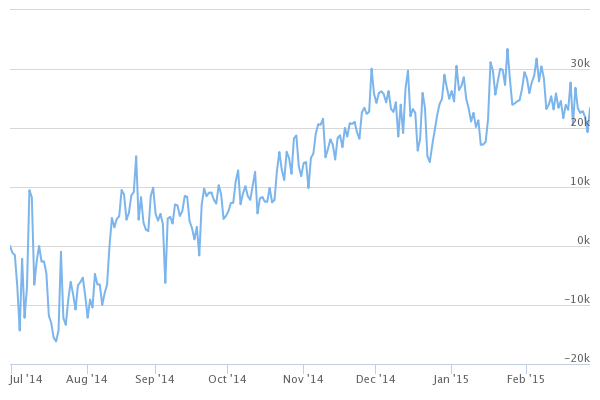
\includegraphics[width=0.8\linewidth]{../img/Leistung.png}
  \caption{Rate of heat flow in watts}
  %\label{fig:}
\end{figure}

\begin{figure}[H]
  \centering
  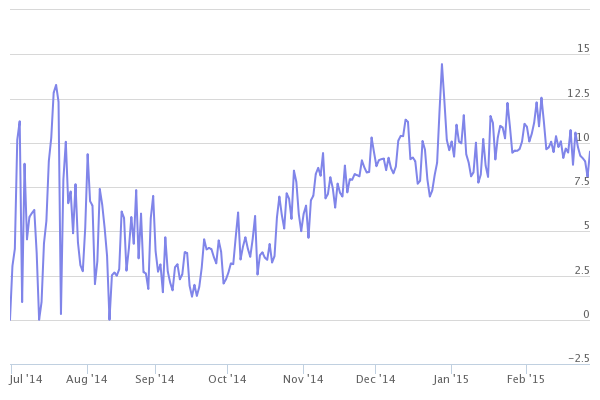
\includegraphics[width=0.8\linewidth]{../img/Volumenstrom.png}
  \caption{Volumetric flow rate in $m^3 / s$}
  %\label{fig:}
\end{figure}


\begin{figure}[H]
  \centering
  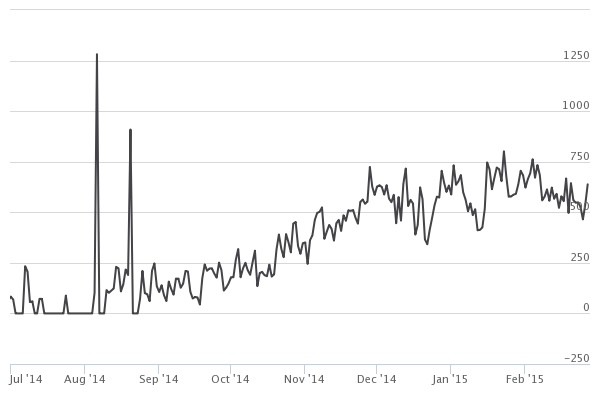
\includegraphics[width=0.8\linewidth]{../img/Energie.png}
  \caption{The Energy in $Nm$ in calculated per day}
  %\label{fig:}
\end{figure}

\begin{figure}[H]
  \centering
  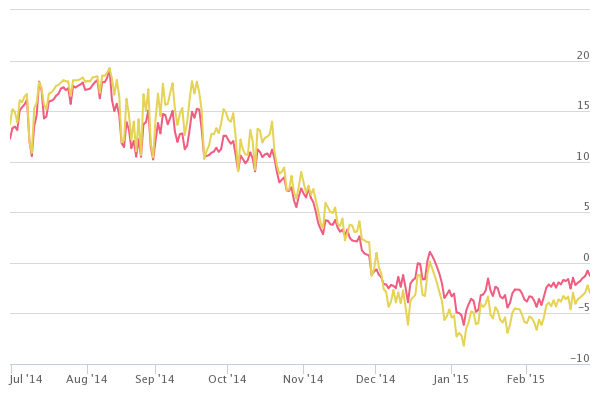
\includegraphics[width=0.8\linewidth]{../img/lauftemperature.png}
  \caption{Supply-(red) and return temperature (yellow) in $^\circ C$}
  %\label{fig:}
\end{figure}

\begin{figure}[H]
  \centering
  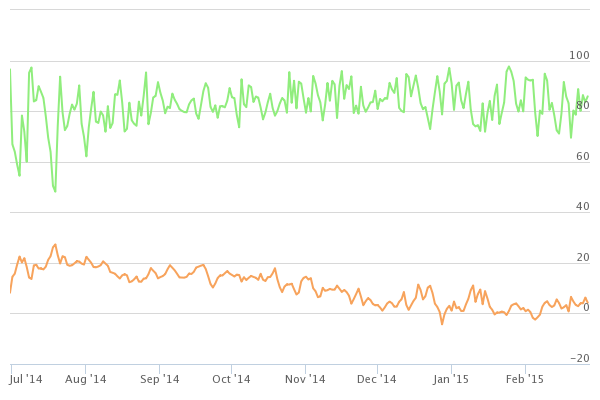
\includegraphics[width=0.8\linewidth]{../img/temp_feuchte.png}
  \caption{Outside temperature in $^\circ C$ (green) and relative air humidity in percent(orange)}
  %\label{fig:}
\end{figure}

\begin{figure}[H]
  \centering
  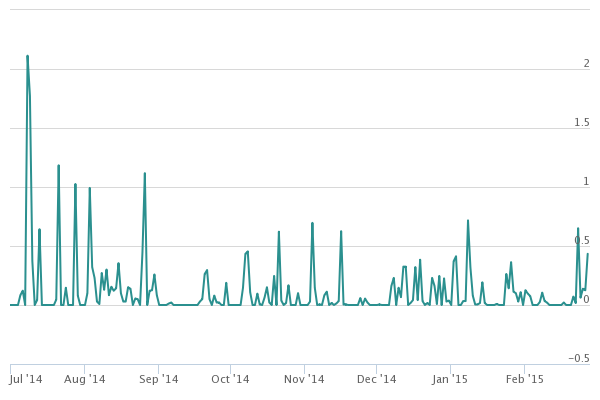
\includegraphics[width=0.8\linewidth]{../img/niederschlag.png}
  \caption{Precipitation in mm (1 litre per square meter)}
  %\label{fig:}
\end{figure}

\subsection{Comments}
As the figures show, the behaviour of the system changed quite dramatically over the time. Hence it is not sure whether a prediction can handle this change.
%CONTENTS
%NOTES


%COPY AND PASTE FROM HERE

%\begin{enumerate}
% \item
%\end{enumerate}

%\href{link}{text}

%\begin[Language=Python]{lstlisting}
%#PYTHON CODE HERE
%\end{lstlisting}

%\lstinputlisting[language=Python]{	}

%\csvautotabular[separator=semicolon]{data.csv}

%\subsubsection{left}
%\begin{figure}[H]
%  \centering
%  \includegraphics[width=0.5\linewidth]{../img/	}
%  %\caption{}
%  %\label{fig:}
%\end{figure}
%PUT UNITS ON THE FIGURES

%BIBLIOGRPAHY?
%\bibliographystyle{plain}%amsalpha
%\bibliography{Top30.bib}
%\bibentry{}

\end{document}
